\section{Bayesian Statistics for HistFactory Models} \label{BayesForpyhf}


\subsection{\texttt{HistFactory} Models and \texttt{pyhf}} \label{subsec:HFandpyhf}

In the \texttt{HistFactory} template, the expected event rates $\nu$ are dependent on two sets of parameters, free parameters $\eta$ and constraint parameters $\chi$. In contrast to the free parameters, the $\chi$ are constrained by external data, whose impact has to be considered when building the statistical model. This can be done by assuming auxiliary measurements with observations $a_{\chi}$ for each parameter $\chi$. Each auxiliary measurement then corresponds to a constraint term  $c_{\chi}$ which is added to the likelihood and controls the compatibility of the value of the constraint parameter $\chi$ with their corresponding auxiliary measurements $a_{\chi}$~\cite{pyhf, pyhf_joss, Cranmer:1456844}. For simplicity, the model for these auxiliary measurements are either Gaussian or Poisson distributions. \\
Taking the constraints into account, the resulting statistical model for event rates $n$ and auxiliary measurements $a$ is then given by~\cite{pyhf, pyhf_joss}:

    \begin{align}
    \begin{split}
        p(x | \theta ) &= p_{\text{main}} (x_{\text{main}}| \theta ) p_{\text{aux}} (x_{\text{aux}}| \theta) \\
         &= p( n, a | \eta, \chi) = \prod_{c \in \text{channels}}  \prod_{b \in \text{bins}} \text{Poiss}(n_{cb} | \nu_{cb}(\eta, \chi)) \prod_{\chi}c_{\chi}(a_{\chi} | \chi),
    \end{split}
    \end{align}

\noindent where $p_{\text{main}}$ ($p_{\text{aux}}$) and $x_{\text{main}}$ ($x_{\text{main}}$) describe the actual and auxiliary statistical model and observations for parameters $\theta$. \\ \\
\noindent The pure-Python library \texttt{pyhf} implements the \texttt{HistFactory} formalism for the analysis of multi-channel binned statistical models~\cite{pyhf, pyhf_joss}. Statistical models can be stored as pure JSON files, allowing for integration with other statistics libraries. The numeric backend that $\pyhf$ uses is flexible, allowing for auto-differentiable tensor-backends.

\subsection{Bayes' Theorem}
Bayesian inference is governed by Bayes' theorem~\cite{ConjPriorsBerkeley}:
    \begin{align} \label{Bayes}
        p(\eta, \chi \vert x, a) = \frac{p(x, a\vert \eta, \chi) p(\eta, \chi)}{p(x, a)}.
    \end{align}
 \noindent It describes the updating of a prior probability distribution $p(\eta, \chi)$ to a posterior distribution $p(\eta, \chi \vert x)$ by multiplication with a data-generating model $p(x \vert \eta, \chi)$. $\eta, \chi$ are parameters of interest (POI) and constraint parameters respectively and $x, a$ observations and auxiliary measurements and evidence $p(x, a)$. While a closed form solution of Eq.~\eqref{Bayes} is intractable due to the evidence, approximate solutions are viable via sampling methods (such as MCMC~\cite{PyMC}) as only a tractable joint likelihood $p(x, a \vert \eta, \chi)p(\eta, \chi)$ is required.

\subsection{\texttt{PyMC}}
\texttt{PyMC} is a Python library for building Bayesian models and already includes a wide range of cross-checks and plotting functions through its \texttt{arviz}-backend~\cite{PyMC, arviz}. \\
\noindent The statistical models are evaluated using Monte Carlo chain methods (MCMC), where the posterior is represented by sampling from the prior distribution steered by the likelihood.
\noindent \texttt{PyMC} also allows for the implementation of external models, which makes it suitable for performing Bayesian inference with \texttt{pyhf}-based \texttt{HistFactory} models. \\
Within \texttt{PyMC} a whole set of MCMC techniques is available, e.g. prior and posterior sampling or predictive sampling. The returned objects are \texttt{arviz.InferenceData} containers, for which again the whole set of analytic tools provided by the \texttt{arviz} library are available~\cite{arviz}.


\subsection{Prior Constraints from Auxiliary Measurements and Ur-Priors}

In order to get a sampling representation of the posterior using MCMC methods the prior distribution and the \texttt{HistFactory} models are needed, i.e following Eq.~\eqref{Bayes}:
    \begin{align}
        p(\eta, \chi \vert x, a) \approx p(x, a \vert \eta, \chi)p(\eta, \chi).
    \end{align}
\noindent While $p(x, a \vert \eta, \chi)$ can be build using \texttt{pyhf}, the prior beliefs of the value of the parameters still have to be quantified. It would be possible to treat $\eta$ and $\chi$ equally, i.e. to determine some ur-prior $p(\eta, \chi)$ by hand and update with $x$ and $a$ in parallel. Ur-priors describe the belief about the parameter value before taking the observations into account. \\
The approach followed in this work however relies on a different treatment of the constraint priors $p(\chi)$. It is based on separating the auxiliary observations $a$ from the main inference step and using it instead in an initial inference step. In this step, Bayes' theorem is used to update ur-priors $p_\text{ur}(\chi)$ with the auxiliary measurements $a$, thus incorporating the information gained from the auxiliary measurements $a$, see Eq.~\eqref{initialInference}.
    \begin{align} \label{initialInference}
	p(\chi \vert a) \approx p(a \vert \chi) p_{\text{ur}}(\chi)
    \end{align}

\noindent The posteriors $p(\chi \vert a)$ from Eq.~\eqref{initialInference} can then be used as prior belief in the main inference step. \\
This approach is useful, as the number of constraint measurements can get arbitrarily high which would imply high computational cost when updating $p(\eta)$ and $p(\chi)$ together. Splitting the auxiliary update of the constraint parameters into this initial step solves this issue based on the concept of conjugate priors. This concept dictates that for given sets of distributions for the priors and the data-generating model, the posterior distribution is of the same distribution family as the prior and can be given in closed form --- the priors and posteriors are then conjugate. Due to the limited possibilities for the auxiliary measurements (which can be either Gaussian or Poisson distributed), this concept is viable for the constraint parameters with corresponding Gaussian and Gamma distributed ur-priors, see Table~\ref{ConjugatePriors}~\cite{ConjPriorsBerkeley}. The freedom to choose these compatible ur-priors is justified as the priors will be dominated by the auxiliary measurements. Indeed, in the limit of very vague ur-priors the priors are completely dominated by the auxiliary measurements $a$:
    \begin{align}
    \begin{split}
        \sigma_{\text{ur}} \gg \sigma_{\text{aux}} \quad &\longrightarrow \quad  \mu' \rightarrow a, \quad \sigma' \rightarrow \sigma_{\text{aux}}, \\
        \alpha_{\text{ur}}, \beta_{\text{ur}} \rightarrow 0 \quad &\longrightarrow \quad \alpha', \beta' \rightarrow a.
    \end{split}
    \end{align}
As the impact of the auxiliary measurements can now be implemented in closed form, no sampling is needed for the implementation of the knowledge gained from the auxiliary measurements $a$.

    \begin{center}
        \begin{tabular}
        {| c || c | c|}
         \hline
          Posterior & Data-Gen. Model & Ur-Prior \\
         \hline
         \hline
         $\mathcal{N}\left( \chi | \mu',~\sigma'\right)$ &$ \mathcal{N}\left( a | \chi,~\sigma_{\text{aux}}\right)$ & $\mathcal{N}\left( \chi | \mu_{\text{ur}},~\sigma_{\text{ur}}\right)$ \\
        \hline
        $\Gamma\left(\chi |\alpha', \beta'\right)$ & $\text{Poiss}\left( a | \chi \right)$ & $\Gamma\left(\chi |\alpha_{\text{ur}}, \beta_{\text{ur}} \right)$ \\
        \hline
        \end{tabular}
    \captionof{table}{Conjugate priors for Poisson and Normal distributed auxiliary measurements $a$~\cite{ConjPriorsBerkeley, Murphy2007}. \label{ConjugatePriors}}
    \end{center}

\noindent While Table~\ref{ConjugatePriors} fixes the general structure of the posterior distribution (to be used as priors in the main inference), the hyperparameters governing these still have to be determined. \\
For a single auxiliary measurement $a$, the hyperparameters for the Gaussian posteriors of $\chi$ for some given ur-hyperparameters $\mu_{\text{ur}}, \sigma_{\text{ur}}$ follow~\cite{Murphy2007}:

    \begin{align} \label{BayesConj}
        \mu'= \frac{\sigma_{\text{aux}}^2 \sigma_{\text{ur}}^2}{\sigma_{\text{aux}}^2 + \sigma_{\text{ur}}^2} \left( \frac{\mu_{\text{ur}}}{\sigma_{\text{ur}}^2} + \frac{a}{\sigma_{\text{aux}}^2}\right) , \quad \sigma' = \frac{\sigma_{\text{aux}}^2 \sigma_{\text{ur}}^2}{\sigma_{\text{aux}}^2 + \sigma_{\text{ur}}^2},
    \end{align}

\noindent The hyperparameters describing the posterior Gamma distribution for a single auxiliary observation $a$ can for some given ur-hyperparameters $\alpha_{\text{ur}}, \beta_{\text{ur}}$ be derived as:
    \begin{align} \label{PoissonUpdating}
        \alpha' = \alpha_{\text{ur}} + a, \quad \beta' = \beta_{\text{ur}} + 1,
    \end{align}
\noindent In contrast to the Gaussian constraints, the implementation of the Poisson constraints in \texttt{pyhf} comes with the following change of variable:
    \begin{align} \label{}
        \chi  \rightarrow \gamma = \frac{\chi}{a}.
    \end{align}
\noindent Using:
    \begin{align}
        p(\chi) \mathrm{d} \chi = p(\gamma) \mathrm{d} \gamma
    \end{align}
\noindent the posterior Gamma distribution over $\gamma$ is then derived as:
    \begin{align}
    \begin{split}
        p(\gamma | a ) &\approx \Gamma(\chi | \alpha', \beta') \frac{\mathrm{d} \chi}{\mathrm{d} \gamma} = a \frac{\chi^{\alpha'-1}}{\Gamma(\alpha')} \text{e}^{-\beta' a \chi} \\
        &\approx \Gamma(\gamma | \alpha', a\beta') = \Gamma(\gamma | \alpha_{\text{ur}} + a, a(\beta_{\text{ur}} + 1)).
    \end{split}
    \end{align}

\noindent Applying the methods described above to Eq.~\eqref{Bayes}, the final form of Bayes' theorem used in this work then reads:
    \begin{align} \label{BayesConj_final}
        p(\eta, \chi \vert x, a) \propto p(x\vert \eta, \chi) p(\eta) p(\chi | a).
    \end{align}


\subsection{Hamiltonian Monte Carlo Sampling}
\texttt{pyhf} supports auto-differentiation via its \texttt{jax, torch} and \texttt{tensorflow} backends~\cite{pyhf, pyhf_joss, jax2018github, tensorflow2015-whitepaper, paszke2017automatic}. Therefore, the Hamiltonian Monte Carlo (HMC) step method provided by \texttt{PyMC} is viable for analysing \texttt{pyhf} \texttt{HistFactory} models. Details on the HMC sampling method can be found in~\cite{vishnoi2021introduction}. For this work, it is sufficient to point out that HMC relies on the derivatives of the model --- and while this comes with a computational cost, the quality of the drawn samples should be higher compared to other step methods, such as Metropolis-Hastings~\cite{Metropolis1953}. \\ \\
\noindent The quality of MCMC chains can be measured using the autocorrelation length, i.e. the correlation between subsequent samples. Independent samples are necessary to fully express the parameter space. In order to reduce the autocorrelation length, thinning can be applied. In thinned chains, only every $n$th sample is kept in the final chains~\cite{hoyer2017xarray}. Fig.~\ref{autocorr} visualises how the Metropolis-Hastings chains have to be thinned twice as much ($n=12$) compared to the HMC chains ($n=6$) in order to keep the autocorrelation within an acceptable range (see Sec.~\ref{BaysWF} for the model used). Accordingly, in order to produce sampling chains of the same magnitude, the computational cost of the gradient calculation can seen as substituting the cost for drawing twice as many samples for Metropolis-Hastings steps.
    \begin{figure}%[H]
        \centering
        % \captionsetup{justification=centering}
        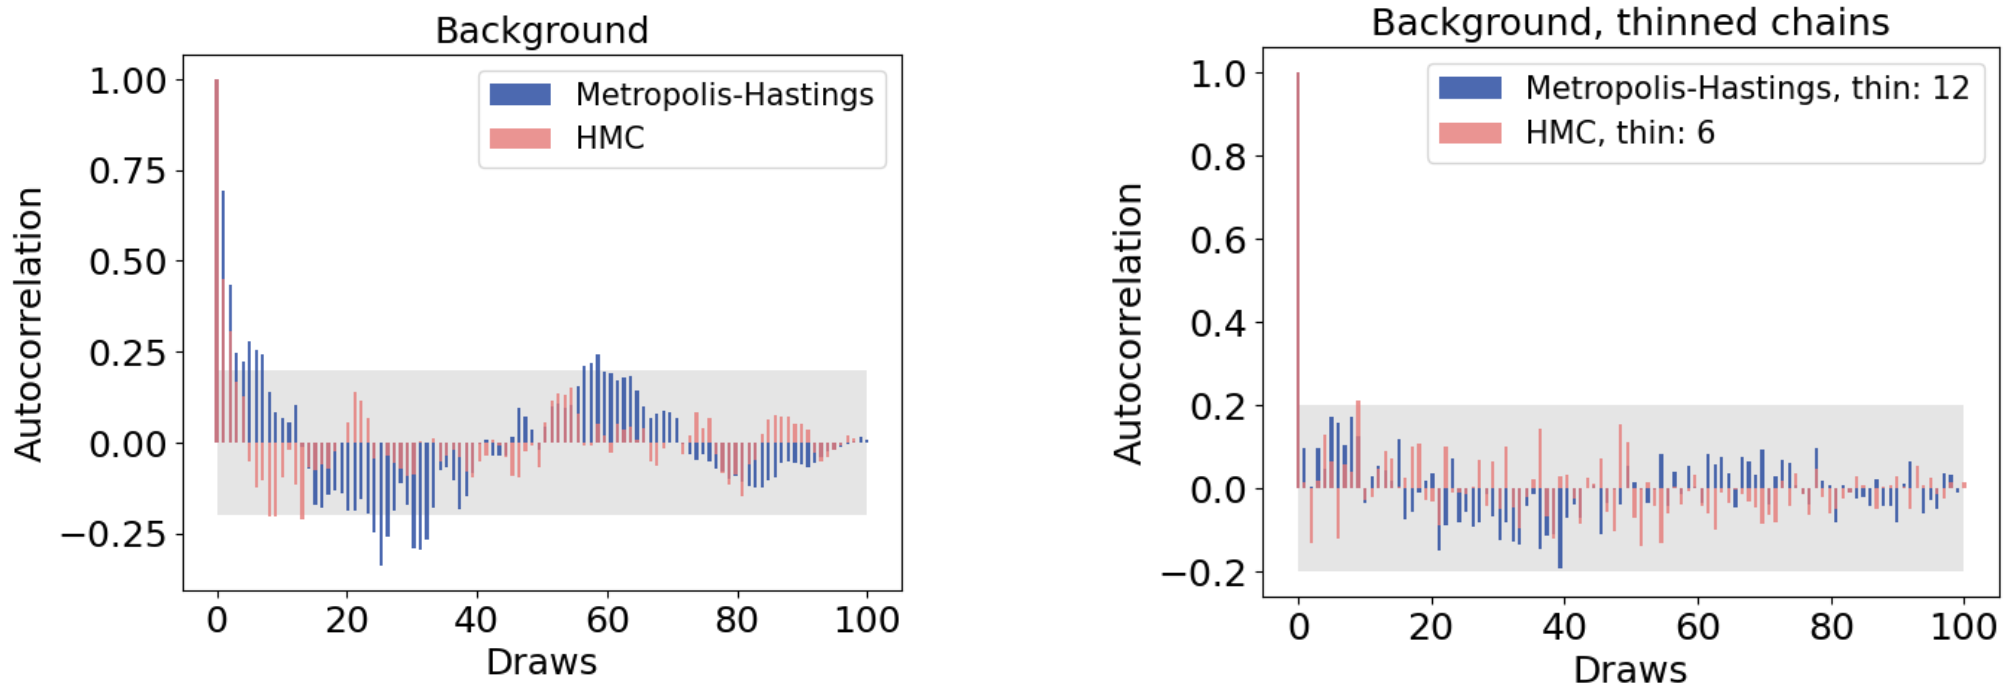
\includegraphics[width=10cm]{figures/autocorr.png}
        \centering
        \caption{Autocorrelation length for the background parameter for HMC and Metropolis-Hastings steps. The left plot shows the original chains, the right the thinned chains. The shaded band indicates the acceptable length.}
        \label{autocorr}
    \end{figure}
